\documentclass{ctuthesis}

\ctusetup{
	xdoctype = B,
	xfaculty = F3,
	mainlanguage = english,
	titlelanguage = english,
	title-english = {Expedition scheduling in an automated warehouse},
	title-czech = {Rozvrhování vyskladňování z automatizovaného skladu},
	specification-file = {zav_prace.pdf},
	front-specification = true,
	department-english = {Department of Computer Science},
	author = {Jan Kalina},
	supervisor = {Ing. Martin Schaefer},
	supervisor-address = {Unknown,\\ Zářivá 232,\\
	  12000 Praha 2},
	  day = 13,
	month = 5,
	year = 2019,
	keywords-english = {scheduling, automated warehouse, optimization, simulation},
}

\ctuprocess

\begin{thanks}

TBD
\end{thanks}

\begin{declaration}

Prohlašuji, že jsem předloženou práci vypracoval
samostatně a že jsem uvedl veškeré použité informační zdroje v souladu
s Metodickým pokynem o dodržování etických principů při přípravě vysokoškolských
závěrečných prací.
\medskip


V Praze, \ctufield{day}.~\monthinlanguage{second}~\ctufield{year}

\end{declaration}
\begin{abstract-english}
This thesis deals with optimization problem of expedition scheduling in an automated warehouse with given set of parameters, requirements and set of items to dispatch in a day. Relevant scheduling problems and their solutions are discussed. Optimization method and objectives are then proposed for the given type of an automated warehouse. Proposed method is implemented in provided simulation tool and evaluated based on it's performance in the simulation.

\end{abstract-english}



\begin{abstract-czech}
test \ldots
\end{abstract-czech} 

\begin{document}

\maketitle

\chapter{Introduction}

Scheduling is a well studied and practical topic. It is widely used in manufacturing facilities, warehouses, which are discussed in this thesis, and many other industries where proper scheduling can play a great role in their success. Despite its importance and years of research, scheduling is quite a challenging problem, especially when it comes to real-world problems where finding an optimal schedule is usually nearly impossible due to its high computational complexity. 

Since the beginning of research in scheduling, many methods and approaches were developed for finding schedules close to optimal schedule in a reasonable time, but what is a good or optimal schedule? Determining the objective of a schedule is a problem on its own. The usual objective of scheduling is to minimize the makespan, which is the length of a schedule, but this objective alone is not sufficient because of the stochastic nature of real-world problems and customized requirements some facility may demand. Many facilities demand different and complex objectives. For example, in case of an automated warehouse, it may be crucial to not only finish expedition in required time but to also expedite items in the required order. 

In this thesis, general methods for solving scheduling problems relevant to scheduling a daily expedition of the given automated warehouse configuration are discussed. Then, method and an objective of a schedule for the given automated warehouse and scenario is proposed and finally proposed method is implemented and evaluated based on results from the provided simulation tool. Basic structure and functionality of an automated warehouse were provided and are described in the upcoming section.

\section{The automated warehouse}

There are many different types of automated warehouses with very different requirements, structures, and functionality. The problem of scheduling an expedition can be very different based on the structure and the type of an automated warehouse. In this thesis, we consider one of the structures of automated warehouses that is fairly common and is based on a real-world problem. 

\subsection{Description}
\label{subsec:Description}
The automated warehouse is part of a factory that produces some items. These items are stored in their warehouse and can be expedited. The automated warehouse has given number of aisles. Each aisle has racks on each side, where items are stored and on each aisle operates a single stacker crane. On one side of each aisle are connected, two conveyors. The first conveyor is moving items from an aisle to one of the expedition ramps, where trucks can be loaded, and the second is bringing in items from production. Before each item reaches an expedition ramp, it needs to be processed by a scanner, which is located at the end of the first conveyor.

When a truck arrives at expedition ramp, stacker cranes should start unloading items on conveyor leading to the expedition ramp. Stacker cranes can move vertically and horizontally in an aisle and can hold a single item each. Stacker crane which has the requested item in its aisle moves to the item grabs it and put it on the conveyor. In case of an item arriving from production to an aisle. Stacker crane on that aisle should take this item and store in a free position in the aisle. Stacker cranes operate automatically and either stores an item from production if it is available or execute scheduled unloadings. If an item arrives from production, stacker cranes prioritize storing an item. It means that as soon as a stacker crane finishes action in progress, it stores an item from production even if it means delaying scheduled unloadings.

Additional details are stated in \ref{sec:Automated warehouse}.

\begin{figure}
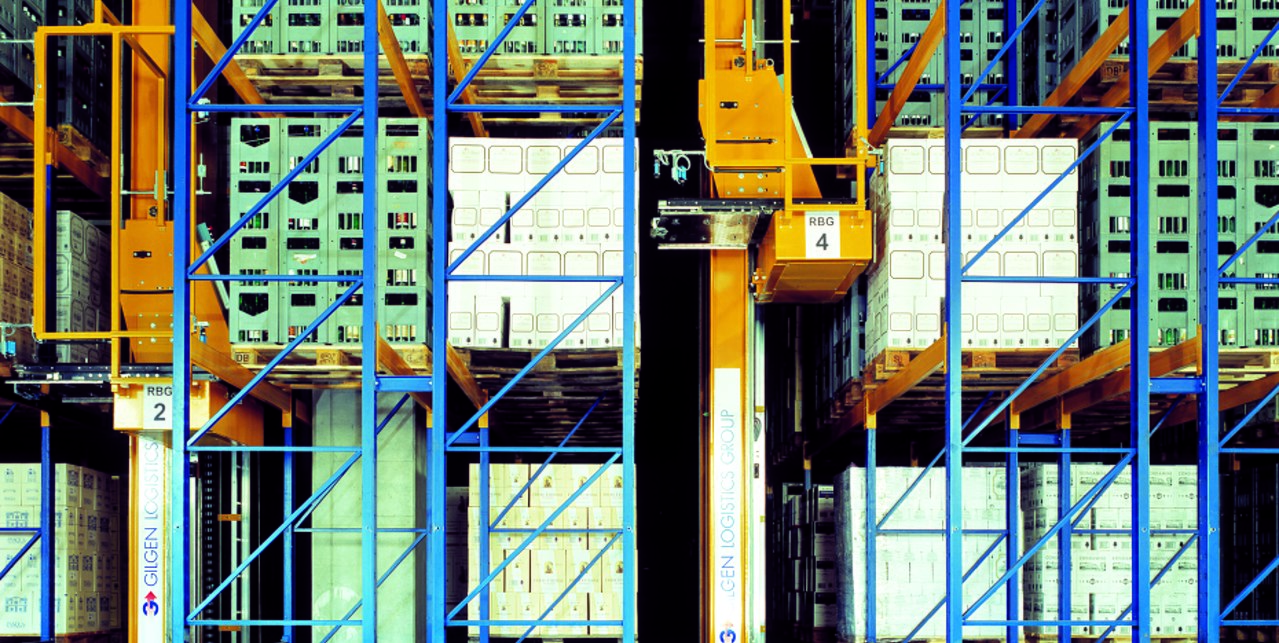
\includegraphics[width=0.8\linewidth]{highbaywarehouse.jpg}
\caption{Example of an automated warehouse with stacker cranes. \cite{warehousepic}}
\label{fig:foobar}
\end{figure}

\section{Motivation}

The goal of this thesis is to be able to create an appropriate schedule in a reasonable time for the given automated warehouse and integrate this schedule to provided simulation tool so that the created schedule can be observed in action and evaluated based on it. With a combination of the schedule and the simulation tool, we are also able to get data about the capabilities of the warehouse itself, which is valuable information when designing an automated warehouse. Integration of the scheduler to the simulation tool also enriches the simulation tool and can be used in future projects.

Properties to consider are prioritization of production handling, limited throughput, and robustness to failure of individual robots. 

\section{Structure of this thesis}



\chapter{Problem statement}
\section{Automated warehouse}
\label{sec:Automated warehouse}

This section describes additional details regarding the warehouse and expedition on top of the description in \ref{subsec:Description} to be able to state scheduling problem properly.

\subsection{Details of the automated warehouse}


Scanners, which are located at the end of every expedition conveyor, accepts an item periodically. Since the scanner is processing items in the given interval, there has to be space between items on conveyor based on the speed of the conveyor and the duration of the interval. If many items arrive too soon after each other, they pile up and may cause the conveyor to stop, which should never happen. To prevent stopping of and conveyor, there is a small buffer. The number of items that pile up in the buffer during a daily expedition will be one of the measurements of robustness to delays.

We also simplify our problem and assume that workers at the loading ramp can always pick up an item coming from the scanner. That means that scanners then create bottlenecks for each expedition ramp where throughput is limited by the frequency at which scanner can process items.

\subsection{Expedition scenario}

We consider expedition is spanned over part of one day. During the expedition, a truck can arrive at an expedition ramp at a scheduled time and demand a certain number of items of different types and order of these types in which they should be loaded into the truck for practical reasons. Items are loaded into a truck in order in which they are processed by a scanner. At each ramp, trucks arrive and leave one after each other. After the expedition of a truck is finished, there is reserved time after which the next truck can arrive to correspond more to reality. 

Which specific items will be expedited is known in advance and is expected that these items are distributed uniformly across all aisles.

\subsection{Available information}

Several basic parameters provided for the given automated warehouse. These parameters include horizontal and vertical speeds and accelerations of stacker cranes, dimensions of a warehouse, speed and length of conveyors, duration of scanning an item, duration of grabbing an item from a conveyor, duration of putting an item on a conveyor and exact location of each item stored in the warehouse. For the expedition, we know count, types, and order at which items should be loaded for each truck. 

From these parameters, we can calculate data needed for describing machine scheduling model.

\section{Notation and terminology}*

\noindent \textbf{Job} ($job_i$) A $job_i$ represents an item $i$ to be expedited. Since expedition items are known in advance $job_i$ is already associated with one of the stacker cranes. 

\noindent \textbf{Machine} ($m_i$) A $m_i$ represents a stacker crane or a scanner. 

\noindent \textbf{Machine processing time} ($p_i$) Time which machine associated with $job_i$ needs to process $job_i$. In other words, time needed to unload an item $i$ from it's location to conveyor. This action consists of trip from conveyor to the item $i$, grabbing the item, trip back to conveyor and putting the item on it. Values of $p_i$ is calculated from speeds, accelerations and dimensions of the warehouse, but if production handling is taken into consideration, these values can become quite inaccurate since stacker crane may not always be at the same spot at the start of a job processing. Processing time is never zero.


\noindent \textbf{Scanning interval} ($s$) Processing time of a scanner. It is equal for every job.

\noindent \textbf{Traverse duration} ($t_i$)

\noindent \textbf{Completion time} ($c_i$)

\noindent \textbf{Completion time of a truck} ($ct_i$)

\noindent \textbf{Start time} ($s_i$)

\noindent \textbf{Reserve}

\noindent \textbf{Stacker crane completion time} ($scc_i$)

\noindent \textbf{Stacker crane start time} ($scs_i$)

\noindent \textbf{Position in expedition} ($pos_i$)

\noindent \textbf{Makespan}

\noindent \textbf{Average flow time}

\noindent \textbf{Total flow time}

\noindent \textbf{TBD - expedition list, ... Add when needed} ($something_i$)


\section{Scheduling problem}
 
 The problem of expedition scheduling in the automated warehouse can be separated into two problems. The first problem is dealing assignment of ramps to trucks and order of trucks at which they arrive. The second problem occurs after the first problem, and it deals with the assignment of completion times to jobs only since machines are predetermined. This thesis mostly tackles the second problem since a good solution to the first problem is fairly easy to get as is shown in chapter \ref{ch:Proposed solution} and scheduling of the second problem has a greater effect on the overall quality of the schedule. *Quality of solution to the 1st problem depends on quality of solution of 2nd problem, address it* 
 
 \subsection{Scheduling trucks}
 
 We will formulate this problem as parallel machine model.
 
 There are $m$ ramps in parallel and $n$ trucks planned for a day. Ramps can be interpreted as machines in parallel and jobs as the whole expedition of each truck. Since each ramp includes only one scanner, which acts are a bottleneck in the warehouse, the objective of this problem is to distribute expedition among ramps uniformly. In other words, workers at each expedition ramp should ideally work the same hours and do the same amount of work.
 
\subsection{Expedition in the automated warehouse as machine scheduling model}

The problem of assigning completion times to jobs in the automated warehouse can be formulated as a special case of 2-stage flexible flow shop (FF2) with blocking or flexible flow line (FFL) with two stages as follows:

There are two work stations connected in series. The first work stations consist of $m$ machines (stacker cranes) in parallel and the second work station consists of $l$ machines (scanners) also in parallel. Every job $job_i$ needs to be processed on its predetermined machine. After job $job_i$ is processed, it travels to a scanner where it needs to be processed too. Jobs cannot wait between work stations, and machines need to start processing a job as soon as it arrives. That alone is referred to as FFL.

Alternatively, we can formulate this problem (with single expedition ramp) as a linear program, as follows:\\
\textbf{Decision variables}

\begin{itemize}
\item $x_{ij}$: 1 if $job_i$ expedited immediately after $job_j$, 0 otherwise
\item$c_i$: completion time of $job_i$ on the second stage
\item$idle_i$: idle time followed after $job_i$ on the second stage
\item$y_i$: order number of $job_i$ on the second stage
\item$scc_i$: start time of $job_i$ on the first stage 
\end{itemize}
\textbf{Data}
\begin{itemize}
\item$p_i$: processing time of $job_i$ on the first stage
\item$E_i$: set of allowed order numbers on the second stage for $job_i$
\item$I_i$: set of indexes of jobs scheduled on machine $i$ on the first stage
\item$M$: represents a large number
\item$start$: time at which work hours start
\item$end$: time at which work hours end
\end{itemize}

\begin{equation}
\begin{aligned}
&\text{minimize}
&&f(\ldots)
\end{aligned}
\end{equation}
\begin{equation}
\begin{aligned}
\text{subject to}\\
& \sum_{i=0}^{n} x_{ij} = 1 &&\\
& c_{i} - c_{j} + M(1 - x_{ij}) \geq s + idle_{i} && \text{for}\; i,j = 1, \ldots, n\\
& c_{i} - scc_{i0} = p_{i} + t_i + s + idle_i && \text{for}\; i = 1, \ldots, n\\
& scc_{i} + p_i < scc_j + M(1 - x_{ij}) && k = 0,\ldots,n, i,j \in I_k\\
& y_{i} - y_{j} < c_i - c_j + M(1 - x_{ij}) && \text{for}\; i,j = 1, \ldots, n\\
& y_i \in E_i && \text{for}\; i = 1, \ldots, n\\
& x_{ij} \in \{0, 1\}  && \text{for}\; i,j = 1, \ldots, n\\ 
& c_i \geq start && \text{for}\; i = 1, \ldots, n\\
& c_i \leq end && \text{for}\; i = 1, \ldots, n\\
& scc_{i} \geq start - p_i && \text{for}\; i = 1, \ldots, n\\
& idle_i \geq 0 && \text{for}\; i = 1, \ldots, n\\
\end{aligned}
\end{equation}
\\

Main requirements of this problem are to make a schedule that fits into working hours of the warehouse and make the schedule robust to random events. For example, the arrival of an item from production can postpone scheduled job at a machine for a whole duration of storing the item, and that can lead to loading items in the wrong order and filling buffer at a scanner. 

In this thesis, objective of this problem is described as minimization of sum of weighted sub-objectives.

Objective:

\begin{equation}
    score = \alpha T + \beta R + \gamma  U
\end{equation}

Sub-objectives:

\begin{enumerate}
\item \textbf{Tardiness} $(T)$\\ \begin{equation}\max(\max_{i=0,\ldots,n}( c_i - end), 0)\end{equation}
why*
\item \textbf{Weighted sum of idle times} $(R)$\\ 
\begin{equation}
    \sum_{i=0}^{n} w_iidle_i
\end{equation}
why*
\item \textbf{Average flow time of trucks} $(U)$
\begin{equation} 
    \dfrac{\sum_{k=0}^{m} \sum_{i \in I_k} c_i}{m}
\end{equation}
why*
\end{enumerate}

 These objectives were selected mostly based on reading on objective functions and robustness in \cite{pinedo} and \cite{tkindt}* and experimenting in the simulation tool. 
 
 Experimenting with these objectives, their effect and trade-off between them is shown in chapter \ref{ch:Evaluation}.

\chapter{Related work}
\label{chap:Related work}
Methods for solving various forms of scheduling problems were extensively studied for decades now. Many of these methods are summarized in \cite{pinedo} and \cite{bucker}. We will mainly discuss methods that are applicable to the flexible flow line and parallel machine problem, which are relevant for this thesis. 

\section{Overview of methods and approaches for finding optimal or nearly optimal schedule}

Both problems we consider in this thesis are NP-hard \cite{complexity} and finding an optimal solution is not an easy task. For finding optimal schedule, seemingly two general methods are used, Linear Integer Programming (LP) and Constraint Programming (CP) with combination of Branch-and-Bound methods, approximation of initial bounds, etc.. LP approach is often obsolete for real-world problems, where there are hundreds or thousands jobs to schedule. CP is in many cases similar to LP, but offers better flexibility for designing constraints and can be optimized for specific problems and because of it it often outperforms LP.

*I will describe CP here

*There are few special cases where optimal schedule can be obtained using some constructing heuristics. 

In following sections, methods for our problems that are often used in literature are discussed.

\subsection{Parallel machine model}

There are few construction heuristics from which we can construct a schedule that guarantees an upper bound of the makespan \cite{gram}. One of these heuristics is The Longest Processing Time first (LPT) heuristics \cite{pinedo} that guarantees that \cite{gram1969}:

\begin{equation}
\dfrac{C_{max}(LPT)}{C_{max}(OPTIMAL)} \leq \dfrac{4}{3} - \dfrac{1}{3m}
\end{equation}

Where $m$ is number of parallel machines.

There are heuristics with slightly tighter bounds and are useful for problems with many jobs, many machines or both. I 

\subsection{Flexible flow line model}

For small instances or simple cases of scheduling problem there often exists dispatching rules from which we are able to construct optimal schedule for objectives like makespan or total flow time. For many practical problems or uncommon objectives, it is hard to recognize 

\section{Value of finding optimal solution}
Finding optimal solution is not really worth it in real world problems. Furthermore solving these problems with CSP or LP requires too much processing time. Even in literature they are saying that around 50 jobs is the limit. 
\section{Solving scheduling problems in practice}
In practice solution is usually constructed using some simple heuristics. Complex heuristics is not really worth using because of random events. Questions usually is what should I try to improve and what heuristics should be good for that. 

FFLL 
\chapter{Proposed solution}
\label{ch:Proposed solution}

The proposed algorithm is designed in a way so that it is simple and fast so that it can be easily applicable in practice and the provided simulation tool.

It consists of four different phases.

\begin{enumerate}
    \item Truck allocation
    \item Job dispatching
    \item Idle time insertion
    \item Re-ordering
\end{enumerate}

As mentioned in \ref{simplicity}, focusing on optimality of a schedule rather than simplicity does not perform well in practice. That being said, in the first phase algorithm optimally assign trucks to ramps. In the second phase, however, heuristic construction is used to get good feasible solution in relatively short time. In the third phase, we insert idle times in between completion time $c_i$ to achieve good robustness to delays caused by prioritized production handling. The last phase is used to further improve on assignments or insertion second and third phases did.

\section{Truck allocation}

\subsection{Objective}

Goal of this stage is to distribute trucks among expedition ramps so that workers at each ramp work almost the same time and do the same amount of work. In other words this can be formulated as minimization of makespan. By minimizing the makespan, we achieve a balanced load among expedition ramps which often leads to good utilization of machines or in our cases expedition ramps \cite{pinedo}. 

 Objective function:
 
 \begin{equation}
     \min(\max(ct_0, ct_1, \ldots, ct_n))
 \end{equation}
 
 *If we take only quantity, works at each ramp do almost the same amount of work. If we take average processing time and setup times, workers work the same hours, but workers at some ramps may be slacking. Weighted duration and processing time seems most reasonable.

\subsection{Algorithm}

In many factories as well as in the automated warehouse, there are not many scheduled trucks in a day (under 50). On top of that, it's objective and problem description is very simple. This makes this problem a good example where CP or LP is effective. Even for it being a real-world problem, finding optimal solution for this case is valuable since stochastic events like "need to reschedule a truck to different ramp" or "truck needs more or less items than it originally demanded" do not occur very often.

This problem of distributing trucks among ramps can be formulated as LP and CP problem as follows:\\

\noindent \textbf{Decision variables}

\begin{itemize}
\item $x_{ij}$: 1 if truck $i$ is assigned to ramp $j$, 0 otherwise
\item$ct_i$: completion time of expedition on a ramp $i$
\end{itemize}
\textbf{Data}
\begin{itemize}
\item$d_i$: approximation of expedition duration of a truck $i$
\end{itemize}

Since the duration of the truck expedition is unknown, we approximate its duration using average processing times $\overline{p}$ as follows:

\begin{equation}
     duration = quantity \cdot \overline{p} + reserve
\end{equation}
 
\subsubsection{LP Model}

\begin{equation}
\begin{aligned}
\text{minimize}\\
&&\max(ct_0, ct_1, \ldots, ct_m)
\end{aligned}
\end{equation}
\begin{equation}
\begin{aligned}
\text{subject to}\\
& \sum_{i=0}^{n} x_{ij} = 1 &&\\
& d_0x_{0j} + d_1x_{1j} + \ldots + d_nx_{nj} = ct_j && \text{for}\; j = 1, \ldots, m\\
\end{aligned}
\end{equation}

\subsubsection{CP model}

\begin{itemize}
    \item Variables:\\
    \begin{equation}
        x_{00}, x_{01}, \ldots, x_{0r}, \ldots, x_{nm}
    \end{equation}
    \begin{equation}
        ct_0, \ldots, ct_m
    \end{equation}
    \item Domains\\
    \begin{equation}
    x_{ij} \in \{0, 1\}
    \end{equation}
    \begin{equation}
    ct_{i} \in \{ d_i, d_i + step, \ldots, upper\_bound\}
    \end{equation}
    \item Constraints
    \begin{equation}
    \begin{aligned}
    & \sum_{i=0}^{n} x_{ij} = 1 &&\\
    & d_0x_{0j} + d_1x_{1j} + \ldots + d_nx_{nj} = ct_j && \text{for}\; j = 1, \ldots, m\\
    \end{aligned}
    \end{equation}
    \item Objective function\\
    \begin{equation}
        makespan = \max(ct_0, ct_1, \ldots, ct_m)
    \end{equation}
    \item Goal\\
    \begin{equation}
        \min(makespan)
    \end{equation}
\end{itemize}

To improve performance of these methods we need to select upper bound of the objective and variables.

\textbf{Upper bound} is calculated using LPT heuristics mentioned in chapter \ref{chap:Related work}.

\textbf{Lower bound}*

In CP approach, LPT heuristics can also be used for ordering of variables. This way the algorithm redistributes trucks with lower load first, which can lead to uniformly distributed workload faster.


\section{Job dispatching}

Using hybrid cyclic heuristics we can distribute jobs quite equally among machines and also try to minimize makespan or other objectives

\section{Idle time insertion}

Now that we know how long is schedule, we can tell how much time we have until work hours end. We can take this time a distribute it among items as idle times. We cannot just simply postpone jobs by idle time, we have run step 2. again, now with idle times.

\section{Meta-heuristics}
Local search (Tabu, simulated annealing)

In scenario where we have more than one ramp, it's not easy to tell how much time I can distribute as idle time. Simulated annealing with ordered moves is good for distributing idle times among jobs. It can basically replace step 3 of proposed algorithm if it wasn't slower. It's better to use it after step 4 to distribute small timeslots to take advantage of remaining time of expedition.

Another improvement is using tabu search which swaps order number of two items. Some objectives are not easily minimized using some heuristics in step 2 like for example weighted penalty for scheduling two jobs right after each other on a single machine because it can lead to stopping a production

\chapter{Implementation}
\section{Simulation environment}
\section{Scheduler module}
\chapter{Evaluation}
\label{ch:Evaluation}
\section{Performance}
\section{Scenarios}
\section{Comparison}
\subsection{Comparison of plan and behavior in simulation}
Comparing different version (LS, no LS, heuristic 1, heuristic 2, ...) of algorithm too.
\subsection{Effect of objectives?}
Mainly significance of idle times (at scanner or machines)
\chapter{Conclusion}

Lorep ipsum \cite{doe}

\begin{thebibliography}{1}
\bibitem{warehousepic} GILGEN LOGISTICS AG. \emph{Automated high-bay warehouse} [online]. 4 December 2016. Available from: https://commons.wikimedia.org/wiki/File:Automatisches\_Hochregallager\_mit\_Regalbediengeräten.jpg
\bibitem{doe} J. Doe. \emph{Book on foobar.} Publisher X,
 2300.
 \bibitem{gram1969} R.L. Graham (1969) \emph{Bounds on Multiprocessing Timing Anomalies}, SIAM
Journal of Applied Mathematics, Vol. 17, pp. 263–269
\bibitem{complexity} A.H.G. Rinnooy Kan (1976) \emph{Machine Scheduling Problems: Classification,
Complexity and Computations}, Nijhoff, The Hague (as cited in \cite{pinedo})


\end{thebibliography}

\end{document}

